% !TEX encoding = UTF-8 Unicode

\chapter{Introduction}

\section{Human Genetics and the Genetics of Complex Traits}

A central goal of genetics is to understand the contribution of genetic variation to phenotypic variation. The mechanism by which genetic variants contribute to a phenotype is determined by the genetic architecture of the phenotype, however, the underlying rules that determine how genetic variants contribute to phenotype diversity are still not fully known. 

Monogenic traits are determined by genetic variation in one gene whereas complex traits do not have predictable patterns of inheritance and have heterogenous phenotypes. Genetic variation in many genes, as well as interaction of genes with environmental factors typically contribute to complex traits phenotypes. 

Genome wide association studies (GWAS) have been effective in detecting associations between common variants and common diseases since 2005, with publication of the first large GWAS with good coverage of the genome in 2007 from the Wellcome Trust Case Control Consortium \cite{WellcomeTrustCaseControlConsortium:2007do}. 

Although GWAS have resulted in the discovery of thousands of novel associations to hundreds of phenotypes, the loci identified by GWAS explain a small proportion of the estimated heritability of the trait, or the fraction of phenotypic variation in a population that is due to genetic variation. There are many explanations that could account for this ``missing heritability," or the proportion of heritability not accounted for by these significant GWAS loci, including gene-environment interactions, epistatic interactions, inflated heritability estimates, rare variants or structural variants not tagged by GWAS SNPs, or common variants with small effect sizes, and parent of origin effects \cite{Zaitlen2013,Eichler:2010kd,Gibson:2012kc,Zuk:cc}. Heritability of parent of origin effects have been extensively studied in mice \cite{Babak2008,Mott2014,Babak2015,Babak2012} and only beginning to be studied in humans \cite{Laurin:2017jv}. The consistently significant GWAS associations, or ``low-hanging fruit" have been further investigated but there still remains a lot of the genome, or ``mid-hanging fruit," that could contribute to a trait (Figure \ref{fig:fig-01-lowhangingfruit}).

\begin{figure}
\centering
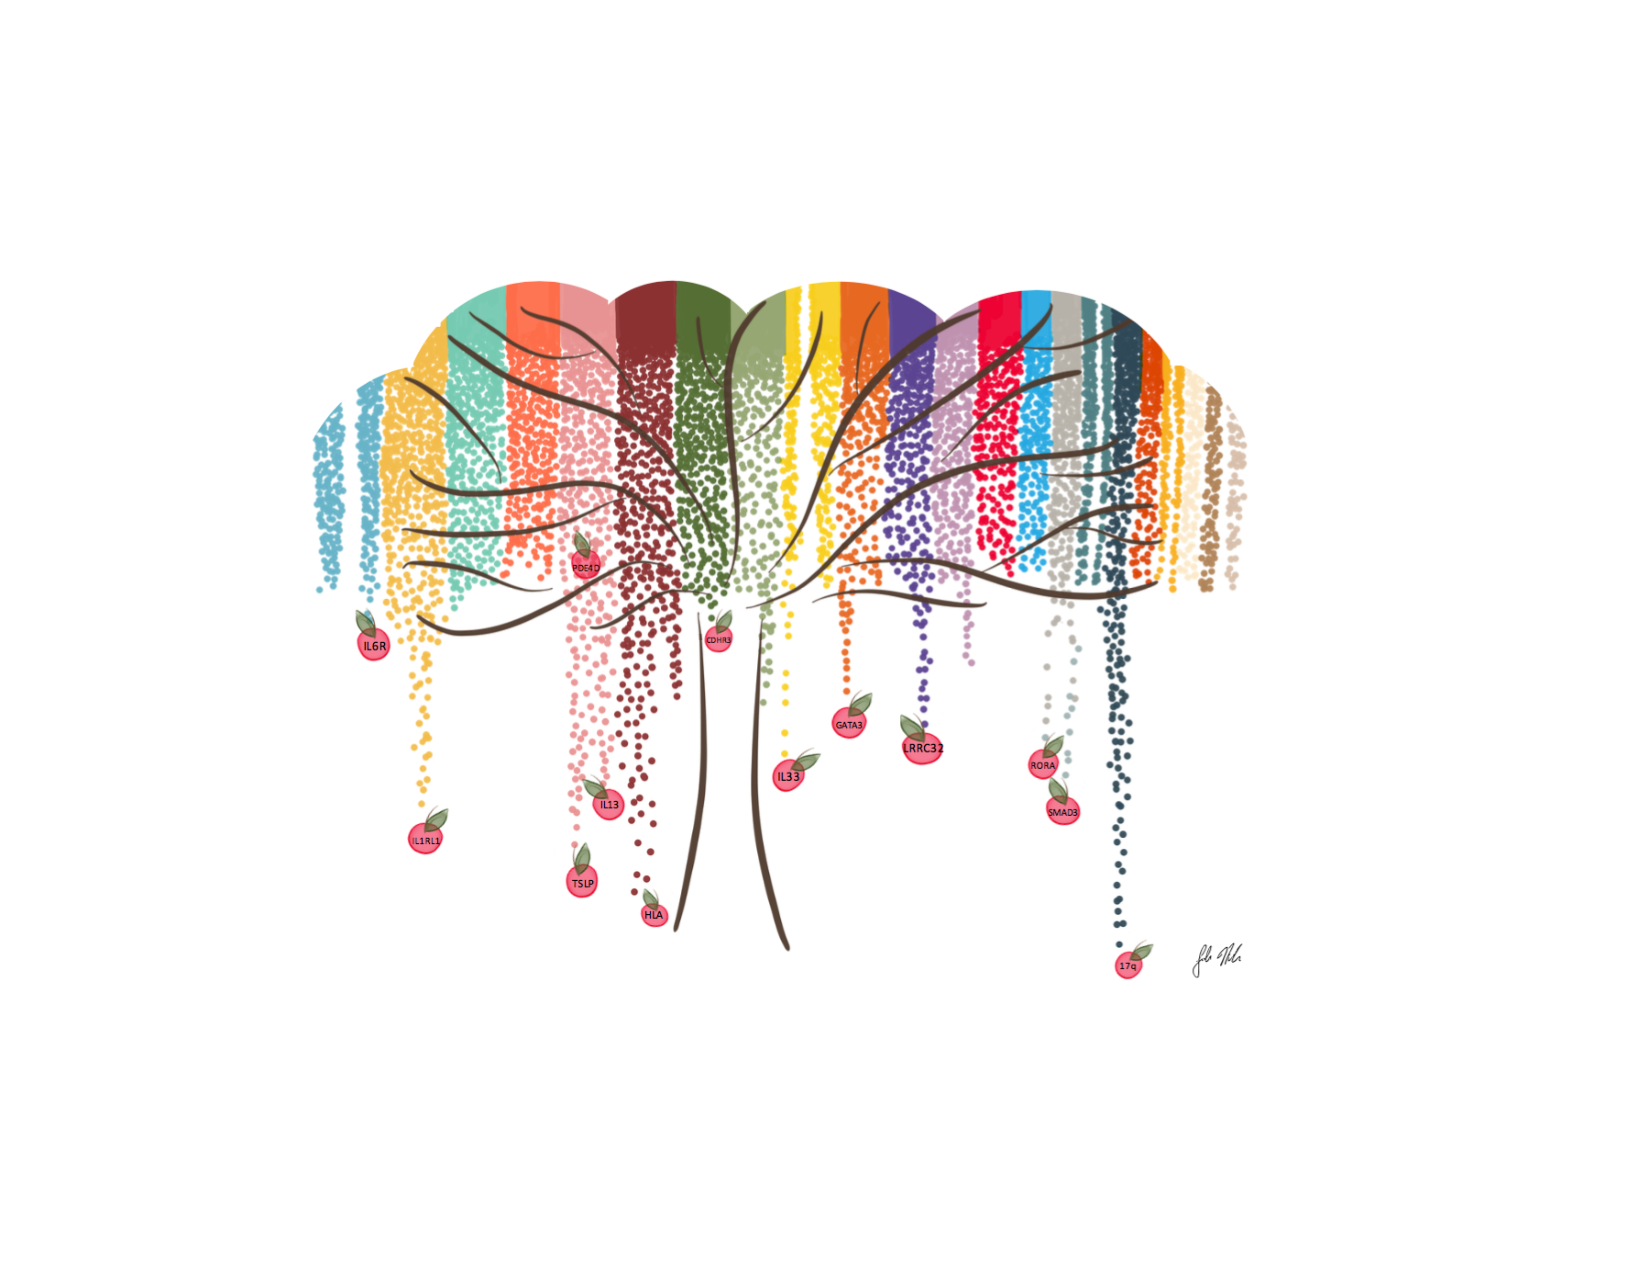
\includegraphics[width=5in]{img/ch01/fig-01-lowhangingfruit.pdf}
\caption[Asthma GWAS Manhattan Plot.]{\textbf{Asthma GWAS Manhattan Plot.} Inverted manhattan plot for asthma GWAS highlighting ``low hanging fruit" as apples hanging from the manhattan plot ``tree." Figure from Ober, 2016 \cite{Ober:2016ga} updated to reflect results from Demenais, 2018 \cite{Demenais:2018hy}.}
\label{fig:fig-01-lowhangingfruit}
\end{figure}

Additionally, in GWAS, the impact of parental origin of associated alleles has been largely ignored, and maternal and paternal alleles are treated as equivalent. Sequence variants could affect disease susceptibility or a quantitative trait differently depending on whether the variant was inherited from the father or the mother. Parent of origin effects include phenomena such as imprinting where epigenetic modifications determined by parental origin allows for differential gene expression of genes on homologous chromosomes \cite{Lokody2014,Lawson2013}. 

The classic examples of parent of origin effects are imprinted genes. More than 80\% of imprinted genes in humans are found in genomic clusters, and at least thirteen clusters have been identified on eight chromosomes \cite{Lawson2013,Peters2014,Pires2014,Abramowitz2012}. These clusters contain both maternally and paternally expressed genes as well as non-coding RNA genes \cite{Peters2014,Abramowitz2012}. Parent-specific expression of the genes within a cluster is determined by cis-acting imprinting control regions (ICRs). ICRs show parental allele-specific DNA methylation and chromatin modifications. ICRs methylated in females during oogenesis typically contain the promoters of long non-coding RNA that are antisense to a protein- coding gene in the cluster and silence it. In contrast, ICRs that acquire methylation in the male germ line are located in intergenic regions.

The testing of maternal and paternal alleles separately can disentangle parent of origin effects. Parent of origin effects can alter gene expression levels that can ultimately affect other phenotypic traits including disease \cite{Lawson2013,Peters2014} . Moreover, parent of origin eQTLs can provide insight into the molecular mechanisms that may underlie genetic associations with both rare and common diseases \cite{Lawson2013,Peters2014,Kong:2009kk,Stridh2014,Falls1999}.



\section{On The Origin of Genomic Imprinting }

Genomic imprinting in its broadest sense suggests that a phenotype observed for a particular gene or genes depends on the sex of the parent from which the gamete containing that gene or genes originated \cite{Sapienza:1989vm}. It was said that a particular gene is imprinted if it results in a different phenotype when it is maternally inherited versus paternally inherited.

The first use of the term``imprinting" was used in reference to the recognition and selective elimination of the paternal chromosomes in \textit{Sciara} \cite{Crouse:1960vc,Sapienza:1989vm}. ``The `imprint' a chromosome bears is unrelated to the genic constitution of the chromosome and is determined only by the sex of the germ line through with the chromosome has been inherited." \cite{Crouse:1960vc} 

The preferential inactivation of the paternally-derived X chromosomes in mouse were the first demonstrations of a functional imprint in mammalian genomes \cite{Takagi:1975ua,Lyon:1984gh,Chandra:1975tb}. Imprinting on autosomes was first suggested by a deletion on mouse chromosome 17 that showed a different phenotype based on which parent the deletion was inherited from \cite{Johnson:1974uf,Johnson:1974kc}. It was not until the development of the pronuclear transplantation technique that allowed for the creation of mice zygotes which contained only maternal or only paternal genetic contributions that there was any evidence that the maternal and paternal genomes are not equal. The differential imprinting on the parental chromosomes prevented complete embryonic development in these mice with complete uniparental disomy \cite{Sapienza:1989vm,McGrath:1984ky}. Parental chromosomes have different regions silenced, or imprinted, such that one parental copy is expressed and having either both parental copies or neither expressed results in genetic and developmental abnormalities.

Further experiments suggested that imprinting occurs during gametogenesis and is necessary for full term development. An egg with a male pronucleus developed to term, but, an egg with two female pronuclei (gynogenetic embryos) or two male pronuclei (androgenetic) developed poorly\cite{Surani1984,McGrath:1984ky}. This provides evidence that input from both parents are required for normal development and the genome of the egg and sperm nuclei are not equal. Non-complementation in genetic crosses of translocated chromosomes provided a way to refine the imprinted regions of the genome\cite{Cattanach:1985hu}. 

Genetic characterization of Prader-Willi syndrome (PWS) was the first human genetic disease to be associated with maternal heterodisomy of chromosome 15q11-13\cite{Nicholls:vh}. It suggested that clinical phenotype of PWS arises from the absence of paternal contribution of 15q11-13 as opposed to a specific genetic mutation. Conversely the absence of maternal contribution to the same region should result in Angelman syndrome (AS) \cite{Nicholls:vh,Reik:1989el}. This provided more evidence that, at ``imprinted" regions, the functional differences depend on the sex of the transmitting parent and genetic input from both parents are required for normal human development \cite{Nicholls:vh}. Various other human imprinted syndromes due to loss or gain of expression of imprinted genes have been characterized summarized in Table \ref{tab:imprinteddisease}.

\begin{table}
\centering
\begin{adjustbox}{width=1\textwidth}
\begin{tabular}{@{}p{3cm}p{2cm}p{7cm}p{7cm}@{}}
\toprule Human Syndrome & Location & Major features & Causes \\ \midrule 
Transient neonatal diabetes mellitus type 1\cite{Mackay:2006bv} & 6q24& Neonatal hyperglycaemia and intrauterine growth restriction & Overexpression of \emph{PLAG1} and \emph{HYMAI}\\
Silver-Russell syndrome\cite{Eggermann:2010gl,Wakeling:2017kv} & 11p15.5 (65\%), MatUPD7  (10\%) & Dysmorphism, intrauterine growth restriction and postnatal growth retardation & Complex: 11p15.5: hypomethylation of \emph{H19} DMR, silencing of \emph{IGF2} and biallelic expression of \emph{H19}; \emph{MEST} and \emph{GRB10} are candidates for MatUPD7 cases\\
Beckwith-Wiedemann syndrome\cite{Choufani:2010ca} & 11p15.5 & Prenatal and or postnatal overgrowth, enlarged tongue, abdominal wall defects, placental overgrowth and predisposition to embryonal tumours. & Complex: mostly epigenetic errors- silencing of \emph{CDKN1C} or biallelic expression \emph{IGF2} and silencing of \emph{H19}; inactivating mutations in \emph{CDKN1C}; PatUPD11\\
Temple Syndrome\cite{Ioannides:2014ka,Kagami:2017gp} / MatUPD14 syndrome & 14q32 & Prenatal and postnatal growth retardation, premature puberty and obesity & Loss of paternal expression of \emph{DLK1} and \emph{RTL1} \\
Kagami-Ogata syndrome\cite{Kagami:2015gn,Kagami:2017gp,Ogata:2016jb} / PatUPD14 syndrome & 14q32 & Dysmorphism, placentomegaly and excessive amniotic fluid & Increased expression of \emph{RTL1}\\
Prader-Willi syndrome\cite{Buiting:2010ci} & 15q11-13 & Developmental delay, obesity, hypogonadism, cognitive impairment & Loss of paternal expression up to 11 genes in 15q11-13 : paternal deletion of MatUPD15\\  
Angelman syndrome\cite{Buiting:2010ci}  & 15q11-13 & Developmental delay, microcephaly, absent or limited speech, gait ataxia, characteristic EEG and behavioral profile with happy demeanour & loss of maternal expression of \emph{UBE3A}, \emph{UBE3A} mutation or patUPD15\\
Mulchandani-Bhoj-Conlin syndrome\cite{Mulchandani:2016kf} & chr15 & Prenatal growth restriction, severe short stature with proportional head circumference, and profound feeding difficulty & MatUPD20\\
Schaaf-Yang syndrome\cite{Fountain:2017dd} & chr15  & deelated psychomotore development, intellectual disability, hypotonia, and behavioral abnormalities & inactivation of \emph{MAGEL2} on paternal allele\\
Central precocious puberty 2\cite{Abreu:2013je} & chr15 & Development of secondary sexual characteristics before age 8 in girls and age 9 in boys. & inactivation of \emph{MKRN3} on paternal allele\\
Pseudo-hypoparathyroidism type 1a and type 1b\cite{Mantovani:2016em,Elli:2016et}  & 20q13.3 & Dysmorphism, obesity, cognitive impairment, end-organ resistance to parathyroid hormone (which results in hypocalcemia and hyperphosphatemia) and resistance to other hormones & Inactivation/lack of maternal \emph{GNAS} \\ 

\bottomrule
\end{tabular}
\end{adjustbox}
\caption[Imprinted Gene Disorders.]{\textbf{Imprinted Gene Disorders.} Adapted from Peters (2014) and Mackay and Temple (2017) \cite{Peters2014,Mackay:2017kn}. UPD = Uniparental Disomy}
\label{tab:imprinteddisease}
\end{table}



\section{The Search for Parent of Origin Effects}


Parent of origin effects and imprinted genes have been most elegantly studied in mice, where two inbred strains are bred reciprocally to identify parent of origin effects on gene expression in progeny that have the same genotypes but different patterns of inheritance \cite{Babak2012}. Such studies are obviously more challenging in humans. Previous studies have attempted to identify parent of origin alleles using different approaches, addressing parent of origin effects on gene expression and phenotypic traits.

In a study of gene expression, investigators examined Hardy Weinberg Equilibrium estimates using genotypes derived from RNA-seq data and considered imprinted loci to be those with no or fewer than expected heterozygotes (C.T. Watson, ASHG 2014). Garg et al. used gene expression in lymphoblastoid cell lines (LCLs) from 29 CEU and 30 YRI HapMap trios to identify 30 imprinting eQTLs with parent of origin specific effects on expression by first comparing maternal alleles and paternal alleles associated with gene expression, and then comparing reciprocal heterozygotes \cite{Garg2012a}. A study from the GTEx Consortium used RNA-seq data to determine allele specific expression (ASE) in 45 different tissues from various numbers of individuals to identify new imprinted genes \cite{Baran:2015cx}. By considering genes with monoallelic expression that were evenly distributed to both the reference and alternate alleles across individuals as evidence for imprinting, they identified 42 imprinted genes, both known and novel, and used family studies to confirm imprinting of 5 novel genes. Most recently, Santoni et al. identified nine novel imprinted genes using single-cell allele-specific gene expression and identifying genes with mono-allelic expression in fibroblasts from 3 unrelated individuals and probands of 2 family trios, and then using the trios to confirm parent of origin of the alleles \cite{Santoni:2017hu}.

Not many studies have searched for parent of origin effects on binary and quantitative traits. In a study on 38,167 Icelanders with known status for 7 diseases, investigators identified variants that were associated with breast cancer when paternally inherited and variants associated with type 2 diabetes when maternally inherited \cite{Kong:2009kk}. Parent of origin associations with height in the same Icelandic population (n=88,835) identified four associations of which three were in known imprinted regions, one of which was also replicated in the Sardinia population \cite{Zoledziewska:2015do}.

\subsection{Dissertation Overview}

Large pedigrees are ideal for identifying parent of origin effects \cite{Baran:2015cx}. The advantages that large family studies have for these studies include: 1) formally proving parent of origin effects detected from ASE, and 2) detecting subtle imprinting that does not lead to strictly monoallelic expression \cite{Baran:2015cx}. The Hutterite population is ideally suited for these studies. The \textgreater 1,400 Hutterite individuals studied by our group are related to each other in a 13-generation pedigree that includes 3,671 individuals, all of whom are descendants of only 64 founders. Ninety-eight Hutterites were initially selected for whole genome sequencing; alleles were phased using Affymetrix framework markers in the 98 individuals and then imputed to the remaining 1,532 Hutterites who had been previously genotyped with the Affymetrix framework markers \cite{Livne2015}. After quality control, parent of origin was assigned to more than 10 million variants. Of the 1,532 with genotype data, 431 also had RNA-seq expression data from LCLs, and between 600-1300 individuals have been phenotyped for cardiovascular disease (CVD) associated  and asthma associated quantitative traits.


In this dissertation, I use a novel variation on GWAS to detect parent of origin effects on quantitative disease-related traits in the Hutterites that would be normally missed in standard GWAS. I am able to find maternal- and paternal-only effects, as well as opposite parent of origin effects. This method can be applied to any quantitative trait for which we know parent of origin of alleles, including gene expression. The method and results of testing this method with quantitative disease related traits is in Chapter \ref{ch:pogwas}. Using LCL gene expression and parent of origin allele information in the Hutterites, I develop a new method of mapping RNA-seq reads to parental haplotypes and detect known and novel imprinted genes in Chapter \ref{ch:imprinted}. The patterns of imprinted genes are validated in a different sample of Hutterite individuals for which we have peripheral blood luekocyte (PBL) RNA-seq and DNA methylation. In Chapter \ref{ch:poeqtl}, I use methods, including one from Chapter \ref{ch:pogwas}, to try and find parent of origin variants that have opposite effects on gene expression. Additionally, we tested for maternal and paternal effects on maternal and paternal gene expression, respectively, and used a parent of origin ASE (PO-ASE) test to identify differences in maternal and paternal gene expression among reciprocal heterozygotes. 

